\documentclass[a4paper,11pt,oneside]{memoir}
\chapterstyle{bianchi} %veelo, culver, crosshead, companion, bianchi

\usepackage{TUINFDA}

\usepackage{url}
\usepackage{hyperref}					% links in pdf
\usepackage{graphicx}            			% Figures
\usepackage{verbatim}            			% Code-Environment
\usepackage[lined,linesnumbered,algochapter]{algorithm2e} % Algorithm-Environment

\usepackage{pgf}					
\usepackage{tikz}					% tikz graphics
\usetikzlibrary{arrows,automata}

\usepackage{ngerman}
\usepackage[ngerman]{babel}
\usepackage{bibgerm,cite}       % Deutsche Bezeichnungen, Automatisches Zusammenfassen von Literaturstellen
\usepackage[ngerman]{varioref}  % Querverweise
% to use the german charset include cp850 for MS-DOS, ansinew for Windows and latin1 for Linux.
% \usepackage[latin1]{inputenc}

\usepackage{scrpage2}
\ifoot[]{}
\cfoot[]{}
\ofoot[\pagemark]{\pagemark}

\pagestyle{scrplain}



\thesistitle{Einsatz von ICT zur Steigerung der Energieeffizienz im landwirtschaftlichen Bereich}
\thesisdate{DD.MM.JJJJ}

\thesisdegree{Bachelor of Science(BSc)}{Bachelor of Science(BSc)}
\thesiscurriculum{Software and Information Engineering}{Software and Information Engineering} % your study
\thesisauthor{Martin Keiblinger} % your name
\thesismatrikelno{0825118} % your registration number

\thesisbetreins{Dipl.-Ing. Mag. Dr. Thomas Neubauer}

% define page numbering styles
\makepagestyle{numberCorner}
\makeevenfoot{numberCorner}{\thepage}{}{}
\makeoddfoot{numberCorner}{}{}{\thepage}

% define custom macros for specific formats or names
\newcommand{\uml}[1]{\texttt{#1}}
\newcommand{\cd}{\textsf{Class Diagram}}

\begin{document}

\captionnamefont{\bfseries}

%%%%%%%%%%%%%%%%%%%%%%%%%%%%%%%%%%%%%%%%%
%%%   FRONTMATTER    %%%%%%%%%%%%%%%%%%%%
%%%%%%%%%%%%%%%%%%%%%%%%%%%%%%%%%%%%%%%%%
\frontmatter
\pagenumbering{roman}

%%%%%%%%%%%%%%%%%%%%%%%%%%%%%%%%%%%%%%%%%
%%%   TITLEPAGES    %%%%%%%%%%%%%%%%%%%%%
%%%%%%%%%%%%%%%%%%%%%%%%%%%%%%%%%%%%%%%%%

% the german title page is required as first page
\selectlanguage{ngerman}

% setup page dimensions for titlepage
\newgeometry{left=2.4cm,right=2.4cm,bottom=2.5cm,top=2cm}

% force baselineskip and parindent
\newlength{\tmpbaselineskip}
\setlength{\tmpbaselineskip}{\baselineskip}
\setlength{\baselineskip}{13.6pt}
\newlength{\tmpparindent}
\setlength{\tmpparindent}{\parindent}
\setlength{\parindent}{17pt}

% first titlepage
\thispagestyle{tuinftitlepage}

%
% Kludge: for each titlepage set \pagenumbering to a different
% style. This is used to fix a problem with hyperref, because there
% are multiple "page 1" and hyperref hates that
%
\pagenumbering{Alph}

\begin{center}
{\ \vspace{4cm}}

\begin{minipage}[t][2.8cm][s]{\textwidth}%
\centering
\thesistitlefontHUGE\sffamily\bfseries\tuinfthesistitle\\
\bigskip
{\thesistitlefonthuge\sffamily\bfseries\tuinfthesissubtitle}
\end{minipage}

\vspace{4cm}

{\thesistitlefontLARGE\sffamily \tuinfthesistype}

\vspace{6mm}

{\thesistitlefontlarge\sffamily von}

\vspace{6mm}

{\thesistitlefontLarge\sffamily\bfseries \tuinfthesisauthor}

\vspace{1.5mm}

{\thesistitlefontlarge\sffamily Matrikelnummer \tuinfthesismatrikelno} 

\vspace{7cm}

\vspace{0pt}\raggedright\thesistitlefontnormalsize\sffamily


\begin{minipage}[t][1cm][t]{\textwidth}%
  \vspace{0pt}\raggedright\thesistitlefontnormalsize\sffamily
  %
  \begin{tabbing}%
	    \hspace{19mm} \= \hspace{66mm} \kill
	    \tuinfthesisbetreuung: \> \tuinfthesisbetreins
  \end{tabbing}
\end{minipage}

\begin{minipage}[t][1.5cm][t]{\textwidth}%
  \vspace{0pt}\sffamily\thesistitlefontnormalsize
  \begin{tabbing}%
    \hspace{35mm}  \kill
    Wien, \tuinfthesisdate  \\    \end{tabbing}
\end{minipage}

\end{center}

% we're done with the titlepages, proceed with default pagenumbering
\pagenumbering{roman}

% restore baselineskip
\setlength{\baselineskip}{\tmpbaselineskip}
\setlength{\parindent}{\tmpparindent}

% back to normal geometry
\restoregeometry

\newgeometry{left=2.5cm,right=2.5cm,bottom=2.5cm,top=2cm}

\selectlanguage{english}

%%% Local Variables:
%%% TeX-PDF-mode: t
%%% TeX-debug-bad-boxes: t
%%% TeX-parse-self: t
%%% TeX-auto-save: t
%%% reftex-plug-into-AUCTeX: t
%%% End:


%%%%%%%%%%%%%%%%%%%%%%%%%%%%%%%%%%%%%%%%%
%%%   ERKLAERUNG DER SELBSTAENDIGKEIT   %
%%%%%%%%%%%%%%%%%%%%%%%%%%%%%%%%%%%%%%%%%

\selectlanguage{ngerman}
\chapter*{Erklärung zur Verfassung der Arbeit}

\tuinfthesisauthor\\
\tuinfthesisauthoraddress

\vspace*{1.2cm}

Hiermit erkläre ich, dass ich diese Arbeit selbständig verfasst habe, 
dass ich die verwendeten Quellen und Hilfsmittel vollständig angegeben 
habe und dass ich die Stellen der Arbeit - einschließlich Tabellen, 
Karten und Abbildungen -, die anderen Werken oder dem Internet im 
Wortlaut oder dem Sinn nach entnommen sind, auf jeden Fall unter Angabe 
der Quelle als Entlehnung kenntlich gemacht habe.\\

\vspace*{2cm}
\begin{tabbing}%
    \hspace{58mm} \= \hspace{28mm} \= \hspace{58mm} \kill
    {\raggedright\rule{58mm}{0.5pt}} \> \> {\raggedright\rule{58mm}{0.5pt}} \\
    \begin{minipage}[t][0.5cm][t]{58mm}
	\vspace{0pt}\sffamily\thesistitlefontnormalsize
	\centering (Ort, Datum)
    \end{minipage}
    \> \>
    \begin{minipage}[t][0.5cm][t]{58mm}
	\vspace{0pt}\sffamily\thesistitlefontnormalsize
	\centering (Unterschrift \tuinfthesisverfassung)
    \end{minipage}
\end{tabbing}


\selectlanguage{english}

%%%%%%%%%%%%%%%%%%%%%%%%%%%%%%%%%%%%%%%%%
%%%   ABSTARCT    %%%%%%%%%%%%%%%%%%%%%%%
%%%%%%%%%%%%%%%%%%%%%%%%%%%%%%%%%%%%%%%%%

\chapter*{Abstract}

Energy efficiency in agriculture is as important as never before. The industrial countries have to work under massive cost pressure whereas developing countries have to compensate their scarcity of resources like watter or electrical energy. The purpose of this work is to give an overview of the the most important research topics for this matter.

The approach for was to find papers which are about the most important research topics defined by the agenda for transnational co-operation on energy efficiency in agriculture of the EU. 

As result this paper shows a survey of papers for mathematical optimization models, sensor network technology, GIS-systems, artificial intelligence and planning systems like decision support systems. The essence of this work is the presentation suitable solutions for optimizing processes and resource consumption. 



%%%%%%%%%%%%%%%%%%%%%%%%%%%%%%%%%%%%%%%%%
%%%   CONTENTS    %%%%%%%%%%%%%%%%%%%%%%%
%%%%%%%%%%%%%%%%%%%%%%%%%%%%%%%%%%%%%%%%%
% uncomment to set document language to german (results in "Inhaltsverzeichnis", "Kapitel", "Abbildung", etc. instead of "Contents", "Chapter", and "Figure"), otherwise the document's language is english
%\selectlanguage{ngerman}

\setcounter{tocdepth}{1}

\cleardoublepage
\pagestyle{numberCorner}
\tableofcontents*

%%%%%%%%%%%%%%%%%%%%%%%%%%%%%%%%%%%%%%%%%
%%%   MAINMATTER    %%%%%%%%%%%%%%%%%%%%%
%%%%%%%%%%%%%%%%%%%%%%%%%%%%%%%%%%%%%%%%%

\mainmatter
\pagenumbering{arabic}
\pagestyle{numberCorner}

%%%%%%%%%%%%%%%%%%%%%%%%%%%%%%%%%%%%%%%%%
\chapter{Einführung}
\label{ch:intro}
%%%%%%%%%%%%%%%%%%%%%%%%%%%%%%%%%%%%%%%%%

\section{Motivation}

Landwirtschaft spielt für jede Gesellschaft eine entscheidende Rolle, da ohne sie die Ernährung der Bürger unmöglich wäre. Für einen Staat ist eine moderne und effiziente Landwirtschaft wichtig um Abhängigkeiten zu anderen Staaten zu verhindern oder zumindest zu verringern. Daher ist dieses Thema auch für Länder der ersten Welt nach wie vor auf der Agenda. Da die Personalkosten hoch sind, ist die Effizenzsteigerung durch Technologie entscheidend für die Entwicklung des Landwirtschaftssektor.

Durch den ständig steigenden Energiebedarf ist vor allem die Frage nach eines optimalen Einsatzes von Energie wichtig für Zukunft der Landwirtschaftsbetriebe in der EU. Neben der Forschung in den Disziplinen der Chemie und des Maschinenbaus, ist die Informatik eine interessante Quelle für kleine und große Optimierungen des landwirtschaftlichen Betriebs. Da ich den Blick über den Tellerrand nicht nur nicht scheue sondern gerne wage und selbst aus einem landwirtschaftlich genutzten Gebiet in Niederösterreich, dem Marchfeld, stamme, liegt mir die Zukunft der Landwirtschaft in Europa am Herzen.

\section{Problemstellung}

Diese Arbeit beschäftigt sich mit der Ausarbeitung des aktuellen Standes der Steigerung der Energieeffizenz in der Landwirtschaft mittels Informations- und Kommunikationstechnik, kurz ICT. Dazu wird eine Zusammenfassung der aktuellen Forschungsprojekte in der EU erstellt und dann eine Zusammenfassung der für Effizenzsteigerung durch ICTs relevanten Literatur erstellt. Dabei wird Wert auf die Ausarbeitung der Forschungsschwerpunkte und Auflistung der für Vergleiche nötigen Kennzahlen. 

Ziel ist es eine Übersicht der relevanten Literatur für folgende Arbeiten zu erstellen.

\section{Verwendete Methode}

Die Quellen für diese Arbeit wurden ohne Fokus auf bestimmte Konfernzen oder Datenbanken ausgewählt. Es wurden alle Arbeiten und Projekte die zumindest innerhalb der EU eine Rolle spielen ausgewertet.

\subsection{Literaturrecherche}
Um möglichst keine relevanten Arbeiten zu übersehen wurden neben den akademischen Datenbanken und Bibliotheken auch Berichte von relevanten Forschungsgruppen der EU herangezogen. Die dort erwähnten Projekte und Arbeiten wurden dann gezielt weiter verfolgt. Für die Suche nach Literatur wurden verschiedene Kombinationen aus folgenden Suchbegriffen gewählt:

\textit{energy, efficency, it, informatic, stochastic, agriculture, Landwirtschaft, Effizenz, ICT, Informationstechnologie, Planung}

\subsection{Selektionsvorgang}
Die wissenschaftliche Literatur wurde auf Basis folgender Kriterien bewertet:
\begin{itemize}
  \item ICT-Relevanz. Bei der Suche nach Effizenz in der Landwirtschaft mussten alle Themen aussortiert werden die sich auf Effizenzsteigerung durch chemische Präparate oder bestimmte Entwicklungen im Maschinenbau bezogen.
  \item Veröffentlichungsmedium. Arbeiten die weder im Rahmen einer Konfernz noch in einem Journals oder zumindestens in einem wissenschaftlichen Magazins veröffentlicht wurden, wurden aussortiert.
  \item Aktualität. Die Arbeiten mussten relativ aktuell sein. Werke die vor 2010 geschrieben wurden, wurden nicht weiter verfolgt.
\end{itemize}

Neben wissenschaftlicher Literatur sind auch Reports von aktuellen Forschungsprojekte eine wichtige Quelle. Bei diesen Projekten wurde ebenfalls auf Aktualität geachtet.

\section{Verwandte Arbeiten}
Eine Übersicht der verschiedenen Forschungsrichtungen wird im Bericht des Projekts D4.5 Agenda for Transnational Co-operation on energy efficency in agriculture geboten.\cite{misc:Mikkola2013}.


%%%%%%%%%%%%%%%%%%%%%%%%%%%%%%%%%%%%%%%%%

%%%%%%%%%%%%%%%%%%%%%%%%%%%%%%%%%%%%%%%%%
\chapter{Datenmodellierung}
\label{ch:dm}
%%%%%%%%%%%%%%%%%%%%%%%%%%%%%%%%%%%%%%%%%

\section{Sichten von Datenmodellen}
Das Modellieren effizienter Datenmodelle spielt in verschiedenen Arten von ICTs eine Rolle. Im folgenden Kapitel wird auf die für Planungs- und Designsysteme relevanten Modellierungen eingegangen. Es wird nicht auf andere Bereiche eingegangen in der Datenmodellierung eine Rolle spielt. Zum Beispiel wäre die Modellierung von Datenstrukturen und Protokollen die erlauben die Daten energiesparend zu verarbeiten, wie es unter anderem in einem Paper von Gang\cite{jour:Lu2007} vorgestellt wurde.

Für Planungs- und Designsysteme dienen dazu, die Betriebswirte in der Bewältigung von Problemen und der langfristigen Planung zu unterstützen. Diese Aufgabe werden in \cite{jour:Schulze2007} in kurzfristige sowie langfristige Planung aufgeteilt. Da sich die Aufgaben und die möglichen Aktionen unterscheiden, wird vorgeschlagen diese auf verschiedene Arten zu modellieren. Dabei werden die kurfristigen Aktionen in der operationalen Sicht, der \textit{Operational View}, und die langfristigen Aktionen in der analytischen Sicht, der \textit{Analytical View}, behandelt. Siehe auch \ref{fig:dataviews}

\begin{figure}[h]
 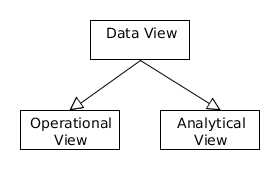
\includegraphics[natwidth=\textwidth]{figures/datamodelling/dataviews.png}
 \centering
 \label{fig:dataviews}
 \caption{Sicht auf Daten. Operational View als Informationsquelle für taktische und Analytical View als Informationsquelle für strategische Entscheidungen.}
\end{figure}

S\o rensen, Fountas und Nash stellen in \cite{jour:Sorensen2010} ein Modell für \textit{Farming Management Information System} kurz FMIS vor. Dies soll als Basis für Planungssysteme wie es aus anderen Branchen als ERP bekannt ist eingesetzt werden. S\o rensen beschreibt dies als drei aufeinander aufbauende Systeme, siehe auch \ref{fig:fmishierarchy}.

\begin{figure}[h]
 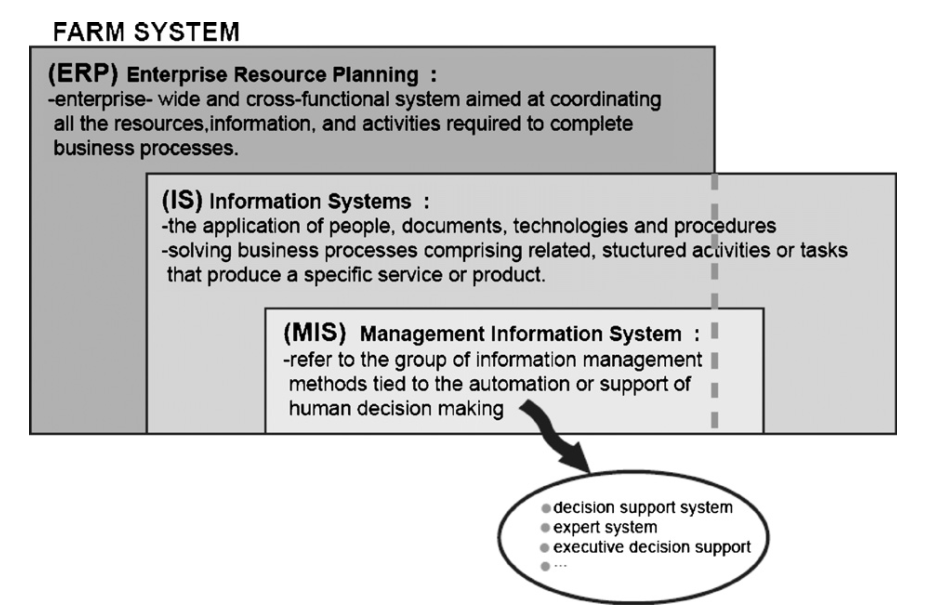
\includegraphics[scale=0.5,natwidth=\textwidth]{figures/datamodelling/sorensen_fmis_2010.png}
 \centering
 \label{fig:fmishierarchy}
 \caption{Konzept eines Management Information Systems.\cite{jour:Sorensen2010}}
\end{figure}

Neben diesen Sichtweisen die für die Entscheidungen im Betrieb wichtig sind, gehen Ruiz-Garcia, Steinberger und Rothmund in \cite{jour:Ruiz-Garcia2010} auf die Modellierung von Daten, Protokollen und Systemen ein, die es erlauben die Verarbeitung der Produkte in allen Schritten der Versorgungskette automatisch überwachen zu lassen. Dies dient dazu, den immer strenger werdenden gesetzlichen Bestimmungen (z.B. der ISO 22005 Standard zur Rückverfolgbarkeit der Lebensmittelbestandteile oder den EU Verordnungen Nr. 178/2002 bzw. Nr. 1935/2004) genügen zu können, ohne die Überprüfungen jedes Lieferanten manuell durchführen zu müssen.

\subsection{Operationale Sicht}
Die operationale Sicht dient dazu Entscheidungen in und für Geschäftsprozesse zu erleichtern bzw. zu ermöglichen. Unternehmerische Geschäftsprozesse werden in \cite{jour:Schulze2007} als Entscheidungen in einem begrenzten Zeitraum beschrieben. Dementsprechend ist es wichtig, dass die operationale Sicht vor allem Daten präsentiert die folgende Bedingungen erfüllen:

\begin{itemize}
	\item Die Daten müssen so aufbereitet werden, dass sie innerhalb der Prozesse verfügbar sind. (\textit{process-orientated data access})
	\item Die Daten müssen aktuell und detailliert sein.
	\item Die Daten müssen Zustände beschreiben. Zustände sollten lt. \cite{jour:Schulze2007} dabei als Menge von Attributen und Relationen zu anderen Zuständen definiert werden.
\end{itemize}

\subsection{Analytische Sicht}
Die analytische Sicht auf die bestehenden Daten leitet sich aus Messungen über einen bestimmten Zeitraum hinweg ab. Als Messungen sind Ergebnisse von bestimmten Berechnungen auf Klassifizierungspfade innerhalb der verfügbaren Datenbasis. In anderen Worten, geht es darum Aggregationen auf Relationen innerhalb von relevanten Ressourcen im Betrieb durchzuführen. Schulze macht dies am Beispiel eines Rinderzuchtsbetriebs für die Milchproduktion deutlich. Dabei werden Informationen über drei Ebenen hinweg aggregiert. So stellt die Sicht auf Ebene der Ställe andere Informationen als auf Ebene der einzelnen Kühe zur Verfügung. Siehe dazu Abbildung \ref{fig:kuehe}. 

\begin{figure}[h]
 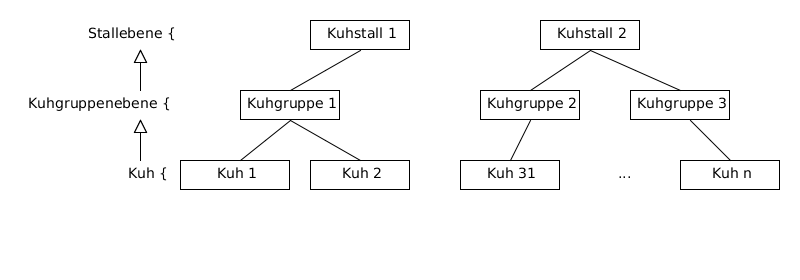
\includegraphics[scale=0.5,natwidth=\textwidth]{figures/datamodelling/kuehe.png}
 \centering
 \label{fig:kuehe}
 \caption{Klassifizierungsschema eines Milcherzeugungsbetriebs.}
\end{figure}

Dadurch wird die analytische Sicht im Unterschied zur operationalen Sicht, durch folgende Eigenschaften definiert:
\begin{itemize}
	\item Die analytische Sicht enthält auch historische Daten.
	\item Die analytische Sicht versucht verschiedene Datenquellen zu integrieren und ein Gesamtbild zu generieren.
	\item Die Daten werden ständig aggregiert und damit wiederverwendet.
\end{itemize}

Multidimensionale Daten können in Form von OLAP-Würfeln visualisiert werden.\ref{fig:kuehe_olap} 

\begin{figure}[h]
 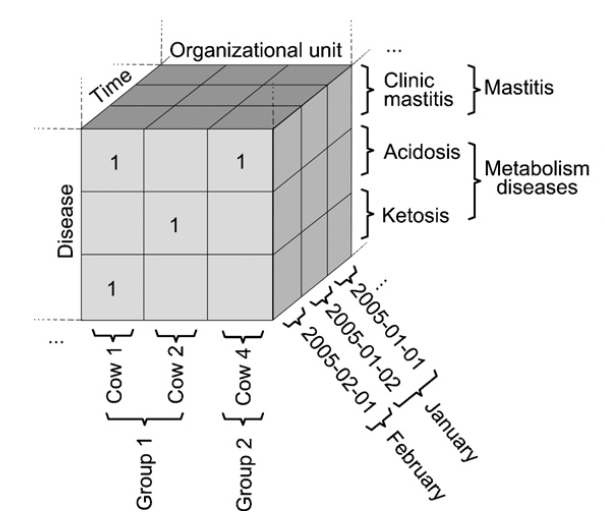
\includegraphics[scale=0.5,natwidth=\textwidth]{figures/datamodelling/kuehe_olap_wuerfel_schulze2007.png}
 \centering
 \label{fig:kuehe_olap}
 \caption{Darstellung der Daten eines Milcherzeugungsbetriebs in Form eines OLAP Würfelns.\cite{jour:Schulze2007}}
\end{figure}

Für die Speicherung und Verarbeitung von solch strukturierten Daten gibt es mehrere Ansätze. Die Daten können entweder getrennt gespeichert und verarbeitet werden in Form der Separierung in OLAP- und OLTP-System, oder auch zusammen geführt werden um die Auswertung auf aktuelleren Daten zu erlauben. Kemper stellt dafür in \cite{jour:Kemper2011} \textit{HyPer} vor.

\section{Entwurf von Datenmodellen}
Das Planen, Entwerfen und Erstellen von Datenmodellen ist ein Prozess, der im Zusammenspiel von Domänenexperten und Datenmodellierungsexperten durchgeführt werden muss. Sowohl S\o rensen wie auch Schulze schlagen dafür einen strukturierten Ansatz vor, der bei der Bestandsaufnahme der Akteure und Ressourcen beginnt und bei der Abbildung der verschiedenen Dimensionen und Relationen endet.\cite{jour:Schulze2007}\cite{jour:Sorensen2010}

Dem oder der Expertin für Datenmodellierung wird dabei nicht nur abverlangt die Relationen und Attribute in den verschiedenen Dimensionen formal abbilden zu können, sondern die Prozesse auch zu identifizieren um sie dann beschreiben zu können. Burkhart, Wolter, Schief, Di Valentin, Werth, Loos und Vaderhaeghen empfehlen dafür eine Ontologie zu entwerfen, stellten aber gleichzeitig fest, dass es noch keine Methode gibt, die völlig zufriedenstellend anleitet.\cite{jour:Burkhart2012} 

Schulz schlägt vor, zur Modellierung der Daten auf ein erweitertes \textit{Entity Relationship Modell}, kurz ER-Modell zurück zu greifen und hat dies auch exemplarisch vorgeführt. 




%%%%%%%%%%%%%%%%%%%%%%%%%%%%%%%%%%%%%%%%%
\chapter{Sensornetzwerke}
\label{ch:intro}
%%%%%%%%%%%%%%%%%%%%%%%%%%%%%%%%%%%%%%%%%

\section{Sensornetzwerke als Datenquellen}
Sensortechnologie wurden im Laufe des AGREE-Projekts zum wichtigsten Forschungsgebiet in der zu zukünftigen Zusammenarbeit gewählt.\cite{misc:Mikkola2013} Sensornetzwerke sind Netzwerke aus Knoten die folgende bestimmte Funktionen verfügen bzw. folgende Bestandteile haben:
\begin{itemize}
	\item Sensoren um verschiedene Umweltparameter messen zu können. (z.B. Luftdruck, Luftfeuchtigkeit, Zusammensetzung der Gase in Umgebungsluft, Helligkeit, etc.)
	\item Rechenmodule um bestimmte Kalkulationen durchzuführen um z.B. Sensorenwerte auszuwerten.
	\item Kommunikationsmodule um entweder Messungen oder (Teil-)Ergebnisse von Kalkulationen zu übermitteln. (z.B. ZigBee, Wireless Lan, etc.)
\end{itemize}
Wenn diese Funktionen um ein Modul zur Fortbewegung des Knotens erweitert wird, handelt es sich um einen mobilen Sensornetzwerkknoten.\cite{jour:Howard2002}

Die Sensormodule können je nach Einsatzzweck sowohl in kleinen, gut zu kontrollierenden Bereichen wie z.B. Glashäusern eingesetzt werden, in großflächigen Feldern oder in Ställen in der Viehhaltung. Dies ist eine notwendige Basis für sg. \textit{Context Aware Computing}-Anlagen die bestimmte Umweltparameter wie z.B. Licht, Nahrung oder Bewässerung steuern können. 

Energieeffizenz spielt für Sensorknoten im Falle von Einsätzen auf großflächigen Feldern eine besondere Rolle, da hier der Einsatz von Batterien bzw. Akkumulatoren eine Notwendigkeit ist und die Wartung bzw. das Austauschen oder Aufladen aufwendig. 

In \textit{Energy Efficient Cognitive Radio MAC Protocols for Adhoc Network: A Survey} werden drei \textit{Media Access Control}-Protokolle, kurz MAC, vorgestellt (ECR-MAC, EECR-MAC, EQR-MAC) die für den Einsatz für Adhoc-Sensornetzwerke konzipiert wurden.\cite{conf:Zia2013} In \textit{Context-Adaptive Multimodal Wireless Sensor
Network for Energy-Efficient Gas Monitoring} werden Optimierung sowohl was das Netzwerkprotokoll bis hin zum Physical Layer betrifft vorgestellt aber auch was den Energiehaushalt des Knoten selbst betrifft. Dabei wird eine Lebenszeit von mehreren Jahren für einen Knoten erreicht.\cite{jour:Jelicic2013}

In \textit{Design and Development of Precision Agriculture System Using Wireless Sensor Network} wird eine Beispiel-Implementierung eines Sensor-Netzwerks zur optimalen Wasserversorgung vorgestellt. Die Autoren kamen zu dem Ergebnis dass sowohl der Ernteertrag gsteigert werden konnte sowie Wasser-, Energie- und Arbeitsaufwand gemindert werden konnten.\cite{jour:Nandurkar2014}

Bhargava untersucht in \textit{Wireless sensor entwork based advisory system for Apple Scab prevention} nicht nur das Netzwerk am effizentesten aufgebaut werden kann, sondern geht auch auf die Auswertung der gemessenen Daten ein. Bhargava unterscheidet hier grob zwischen zwei Architekturen:
\begin{itemize}
	\item Die sg. \textit{Two-Tier-Architecture}
	\item Einem \textit{Peer to Peer Netzwerk} kurz P2P
\end{itemize}

Die Two-Tier-Architektur ist die Aufteilung von Sensor-Netzwerk und Intelligenz. Dabei sind die Tiers durch das Internet verbunden was auch die Auswertung in Cloud-Services erlauben würde. Neben dem Vorteil die Auswertung auch aus dem Betrieb auslagern zu können, erlaubt diese Aufteilung auch die Knoten langlebiger betreiben zu können. Der Autor stellt fest, dass auf den Sensorknoten eine jede Berechnung auf Kosten der verfügbaren Akkuleistung geht.\cite{jour:Bhargava2014}

\begin{figure}[h]
 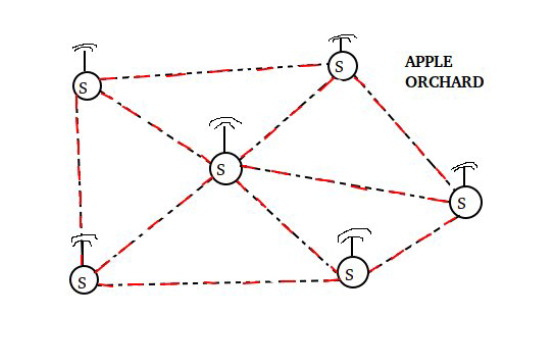
\includegraphics[scale=0.5,natwidth=\textwidth]{figures/sensors/p2p_architecture.png}
 \centering
 \label{fig:fmishierarchy}
 \caption{Vorgeschlagene Two-Tier-Architektur \cite{jour:Bhargava2014}}
\end{figure}

Im Gegensatz dazu, werden die gemessenen Daten in der P2P-Architektur im Netzwerk selbst ausgewertet. Dies hat im Vergleich zur Two-Tier-Architektur einige Nachteile:
\begin{itemize}
	\item Die Lebensdauer der verwendete Energiequelle leidet darunter und ist früher erschöpft.
	\item Es können durch die begrenzte Leistungsfähigkeit der verfügbaren Chips auf den Sensorknoten nur triviale Auswertungen durchgeführt werden.
	\item Je nach Einsatzgebiet (z.B. in gebirgigen Landschaften), kann die Verfügbarkeit der Daten nicht garantiert werden. Dies könnte bei einem Alarm dazu führen, dass dieser nur zu spät gemeldet werden kann.
\end{itemize}

\begin{figure}[h]
 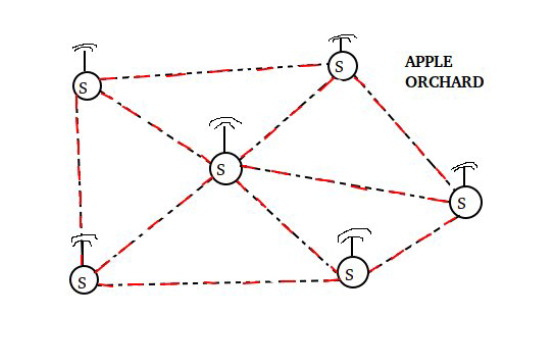
\includegraphics[scale=0.5,natwidth=\textwidth]{figures/sensors/p2p_architecture.png}
 \centering
 \label{fig:fmishierarchy}
 \caption{P2P-Struktur des Sensornetzwerks \cite{jour:Bhargava2014}}
\end{figure}

Aus diesen Gründen spricht Bhargava die Empfehlung aus, die Auswertung auf einen Server welcher über das Internet erreichbar ist auszulagern.\cite{jour:Bhargava2014}

In \textit{Environmental parameters monitoring in precision agriculture using wireless sensor
networks} wird ein Sensornetzwerk für ein Paradeiserglashaus entworfen. Die verwendeten Sensoren maßen die Temperatur, Erdfeuchtigkeit und pH-Wert der Erde. Im Unterschied zu Bhargava wurde ein Gossip-Protokoll zur Kommunikation innerhalb des Sensornetzwerks verwendet.\cite{jour:Srbinovska2014}

Gossip-Protokolle sind definiert durch eine Netzwerktopologie ohne Superknoten. Die einzelnen Knoten besitzen einen lokalen Zustand der im Netzwerk mittels Broadcasts in definierten Abständen mitgeteilt wird. Dies hat zur Folge, dass einzelne Knoten ohne Aufwand hinzugefügt oder entfernt werden können. Dieses Vorgehen hat Vorteile da keine Superknoten benötigt werden die das Routing übernehmen, ist jedoch energieaufwendig. Die Energieaufnahme versucht Pazurkiewicz in \textit{NarrowCast: A New Link-layer Primitive for Gossip-based Sensornet Protocols} mit seinem NarrowCast-Protokol zu mindern.\cite{jour:Pazurkiewicz2014}

Srbinovska und seine Kollegen haben sich für ein Gossip-Protokoll in ihrem Testaufbau entschieden, da für das System ein Temperaturdurchschnittswert interessant ist. Durch die Broadcasts der jeweilig lokal gemessenen Temperaturen wurden lokal auf den Knoten die Durchschnittswerte errechnet und gespeichert. Im Experiment wurde fest gestellt, dass die Durchschnittswerte der einzelnen Knoten annäherend dem tatsächlichen Wert entsprach. Dies dauerte zwischen 15 und 20 Broadcasts.\cite{jour:Srbinovska2014}

Die Autoren kamen abschließend zu dem Ergebnis, dass bei der Planung auf mehrere Aspekte geachtet werden muss.\cite{jour:Srbinovska2014}
\begin{itemize}
	\item Auswahl des effizientesten Frequenzbereichs für die Funkverbindung. Die Frequenz der WiFi-Transmitter ist entscheidend für die Energieeffizenz der Sensor-Knoten.
	\item Die Preise der verfügbaren Hardware-Module ist zu hoch.
	\item Vor dem Ausrollen solcher Sensornetzwerke in großen Anlagen, müssen weitere Pilotprojekte durchgeführt werden um den Erfolg nicht zu gefährden.
\end{itemize}

\section{Satellitensysteme als Datenquellen}

In \textit{Estimating rice nitrogen status with satellite remote sensing in Northeast China} wird eine auf Satellitenbildern aufbauende Analyse des Reisanbaus vorgeschlagen. Dieses Vorgehen hat den Vorteil, dass zum einen die Gebiete nicht mit Sensorknoten bestückt werden müssen - was im Falle von Nassgebieten wie Reisfeldern weitere Probleme bereit hält - und dass die lokalen Messinstrumente nur über längere Zeitperioden verlässliche Daten liefern.\cite{jour:Huang2013} 

\begin{figure}[h]
 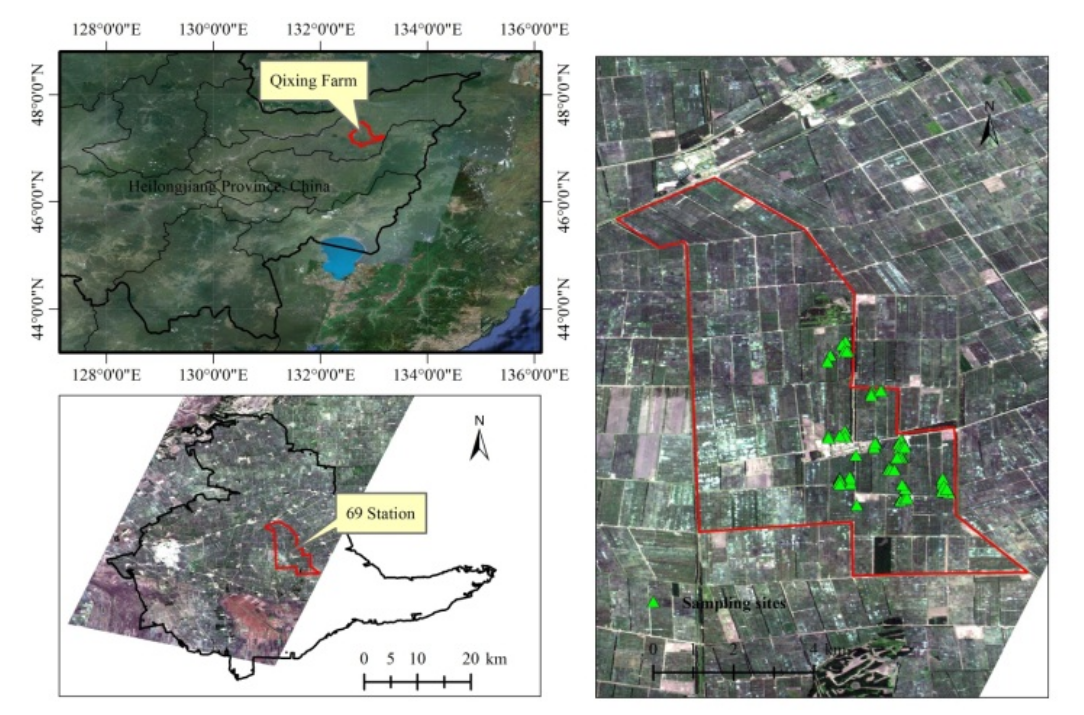
\includegraphics[scale=0.4,natwidth=\textwidth]{figures/sensors/satellite_area.png}
 \centering
 \label{fig:fmishierarchy}
 \caption{Aufnahme des Gebiets dessen Umweltwerte gemessen wurden. \cite{jour:Huang2013}}
\end{figure}


%%%%%%%%%%%%%%%%%%%%%%%%%%%%%%%%%%%%%%%%%

\chapter{Expertensysteme und Design Tools}
\label{ch:intro}
%%%%%%%%%%%%%%%%%%%%%%%%%%%%%%%%%%%%%%%%%


\section{Automatisierte Entscheidungsfindung}

Die ganzheitliche Planung von Landwirtschaftsbetrieben ist ein komplexes Problem das makroskopische sowie mikroskopische Faktoren einbeziehen muss. Ein sehr früher Ansatz um alle Umwelteinflüsse zu bewerten und die Ergebnisse in einer Optimierung der Prozesse infließen zu lassen, ist das \textit{Life Cycle Assessment}, kurz LCA. Dabei werden alle Einflüsse in den Lebenszyklusphasen des Produkts bzw. Services identifiziert. Das Ergebnis dieses Identifikationsprozesses wird \textit{Inventory Table} genannt. Die identifizierten Bestände werden dann mittels \textit{Life Cycle Inventory Impact Assessment}, kurz LCIA oder LCI, auf Zahlen abgebildet die wiederspiegeln wie viel Einfluss die jeweiligen Faktoren haben. LCIA besteht aus vier Schritten:\cite{jour:Klopffer1997}

\begin{itemize}
	\item \textit{Klassifizierung}. Dazu werden die Eingabe- und Ausgabewerte die im \textit{Inventory Table} definiert zusammen gefasst.
	\item \textit{Charakterisierung}. Die im ersten Schritt zusammen gefassten Daten werden dann auf sg. \textit{impact categories}, also Einflusskategorien, abgebildet. Z.B. Sonnenstunden auf Maisertrag.
	\item \textit{Normalisierung}. Die in der Klassifierzung fest gestellten Einflusskategorien werden auf normalisierte Kategorien abgebildet. (Z.B. IPCC-Faktoren für Einflusskategorien der globalen Erwärmung.)
	\item \textit{Bewertung}. In diesem Schritt werden die klassifizierten Kategorien auf ihre Einflussmöglichkeit auf die Qualität des Produkts bzw. Services bewertet.
\end{itemize}

LCA ist auch in dem ISO-Standard 14044 enthalten.\cite{jour:Klopffer1997}

Eine andere Sicht auf die Datenquellen liefern Wang und Pang in \textit{The Design of Protected Agriculture Monitoring Information System
Based on GIS - A Case Study of Qiqihar}. Sie stellen ein System zur Evaluierung der nötigen Informationen, die für Entscheidungen der Landwirtschaft in Qiqihar nötig sind vor. Dabei liegt der Fokus vorallem auf Geschäftsanforderungen die den Rahmen vorgeben was mit den verfügbaren Mitteln erreicht werden. Dabei wird klar, dass die technischen Möglichkeiten, die vorhandene Nachfrage, die Umweltfaktoren sowie gesetzliche Vorlagen beachtet werden müssen. \cite{jour:Wang2013}

\begin{figure}[h]
 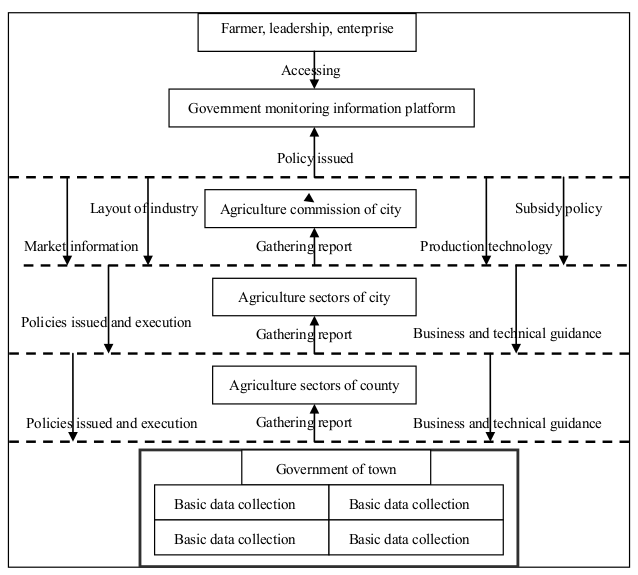
\includegraphics[scale=0.6,natwidth=\textwidth]{figures/designtools/businessrequirements.png}
 \centering
 \label{fig:fmishierarchy}
 \caption{Hierarchie von Datenquellen zu Entscheidungsträgern. \cite{jour:Wang2013}}.
\end{figure}

\subsection{Entwicklungen in der automatischen Auswertung}
Die Möglichkeit LCA in der Landwirtschaft einzusetzen wird in \textit{Streamlining life cycle inventory data generation in agriculture using traceability data and information and communication technologies – part I: concepts and technical basis} beleuchtet. Zu Beginn des Papers gehen die Autoren auf Probleme herkömmlicher LCAs ein:\cite{jour:Bellon-Maurel2014}
\begin{itemize}
	\item LCA als begleitende Maßnahme ist teuer da die Ermittlung der relevanten Daten aufwändig ist. Dementsprechend können nur große Betrieb LCA durchführen.
	\item Die herkömmlichen Messmöglichkeiten ermöglichen nur eine zeitverzögerte Reaktion die im Umfeld der Landwirtschaft zu Ausfällen führen können.
\end{itemize}

In ihrer Arbeit versuchen Bellon-Maurel, Short, Roux, Schulz und Peters den aktuellen Forschungsstand zusammen zu fassen und empfehlen den verstärkten Einsatz von ICTs um die LCI-Prozesse sie auf Kosten und Geschwindigkeit zu optimieren.\cite{jour:Bellon-Maurel2014}

Ein Faktor dessen Optimierungspotential durch Simulation erforscht wurde ist die maximale Lichteffizenz (\textit{maximum light efficency} $\varepsilon_{max}$. Wenquan, Yaozhang, Hao, Deyong und Haibo haben in \textit{Simulation of maximum light use efficiency for some typical vegetation types in China} gezeigt, dass der Fehlerintervall ihres Simulationsmodells klein genug ist um stabile und verlässliche Werte der Primärproduktion, kurz NPP, zu errechnen.  Damit kann bestimmt werden wo bestimmte Pflanzensorten angebaut werden können um den Ertrag zu maximieren. Die Basis für das Modell sind meterologische Daten, Vegetationskarten und vorhandene NPP-Daten.  \cite{jour:Zhu2006}

\subsection{Entwicklungen in Schwellenländern}

In der dritten Welt zeichnet sich durch die Verbreitung von Smartphones einer durch das Mobilfunknetz gestützte Schwarmintelligenz ab. Damit wird die Menge der Kontakte eines Bauers zu einem Orakel, dass zu den Themen Wetter, Ertrag und Best-Practices befragt werden können.\cite{jour:Razaque2013} Die Bedeutung der Übertragung von Informationen für den Ertrag und damit der Effizenz wird in \textit{Assessment of the Role of Mass Media in the Dissemination of Agricultural Technologies among Farmers in Kaduna North Local Government Area of Kaduna State, Nigeria} untersucht. Das Ergebnis war, dass sowohl Internet wie auch Fernsehen und Radio zur Verfügung stehen. Interessant dabei ist, dass in diesen Gebieten hauptsächlich Fernsehen- und Radioübertragung zur Verfügung stehen. Das Potential eine Schwarmintelligenz wie in \cite{jour:razaque2013} beschrieben aufzubauen ist vorhanden.\cite{jour:State2013}

Die Entwicklung der Abdeckung des Mobilfunknetzes in Indien und die gestarteten Projekte zur Steigerung des Ertrags mittels Mobilfunkprojekten wird in \textit{Use of Mobile Technologies for Empowering Small holder farmers in India} vorgestellt. Dabei werden Lösungen wie mKrishi vorgestellt, welches es den Bauern ermöglichen soll per Telephonanruf Fragen bezüglich der Landwirtschaftsarbeit in normaler Sprache zu stellen. \cite{article:Kokate2013}

\section{Expertensysteme in der Planung}
Ein Expertensystem ist ein KI-Programm, dass zwei Rollen annehmen kann.
\begin{itemize}
	\item \textit{Decision Maker}, als Entscheidungsfinder ermittelt das Expertensystem die qualitativ beste Lösung für ein gegebenes Problem. Z.B. die Behandlung eines Patienten mit definierten Symptomen oder die optimiale Bewässerung von Pflanzen.
	\item \textit{Oracle}, in diesem Fall dient das Expertensystem als Entscheidungshilfe in dem es gestellte Fragen beantwortet. 
\end{itemize}
Entscheidend für die Funktionalität des Expertensystems ist, dass ein Kausalmodell für die Problemdomäne gefunden wird, dieses zu einem quantitativen Entscheidungsmodell umgewandelt werden kann und daraus dann eine Entscheidung bzw. Antwort abgeleitet werden kann.\cite{book:Russell1995}

\begin{figure}[h]
 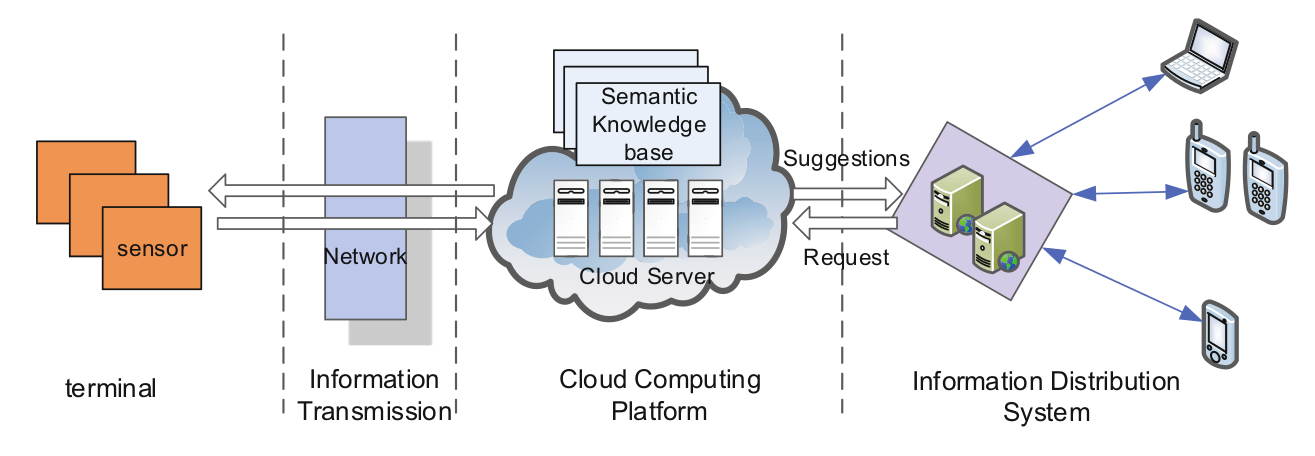
\includegraphics[scale=0.35,natwidth=\textwidth]{figures/designtools/cloud_iot_decisionmaker.png}
 \centering
 \label{fig:fmishierarchy}
 \caption{Architektur der Cloud-basierten Entscheidungshilfe.\cite{jour:Yuan2013}}.
\end{figure}

Lin, Nan, Li, Dongming, Bi und Chunguang stellen in \textit{Research on Development of Corn Production Decision} eine mögliche Architektur für ein System vor, dass bei der Planung und Pflege von Mais helfen soll. Dabei stellen sie folgende Best-Practices vor: 
\cite{jour:Lin2013}

\begin{itemize}
	\item Die Systemarchitektur und die Verwendung müssen als UML-Diagramme abgebildet werden. (Use-Case-Diagramme, Aktivitätsdiagramme, etc.)
	\item Die Datenbankstruktur muss als ER-Diagramm abgebildet werden.
	\item Die nötigen Objekte sollen mit der \textit{Object Definition Language}, kurz ODL, definiert werden.
	\item Die Verwendung der \textit{Framework Representation} um die Hierarchie und damit Kausalität von bestimmten Eigenschaften und Ereignissen abzubilden. (Z.B. ist ein Teil-Frame des Zustands von Gras dessen Halmzustand oder eine Erkrankung Teil des Disaster-Frames.)
\end{itemize}

Das in \textit{A new Expert System for greenness identification in agricultural images} vorgestellte Expertensystem dient dazu, die grüne Färbung der Blätter zu bestimmen. Dies kann z.B. dazu genutzt werden um die Wasserversorgung bedarfsorientiert zu gewährleisten.\cite{jour:Romeo2013}

Um die Entscheidungsfindung besser in puncto Effizienz und Geschwindigkeit zu machen wird in \textit{A Semantic Technology Supported Precision Agriculture System: A Case Study for Citrus Fertilizing} ein Cloud basiertes System vorgestellt. \cite{jour:Yuan2013}

Yuan, Zeng und Zhang stellen in ihrer Arbeit ein Expertensystem auf Basis eines Wissensbasierten System vor. Dabei werden Daten aus einem Sensornetzwerk als Ontologien abgebildet. Diese werden in der Cloud gespeichert. In der Cloud sitzt auch das Expertensystem, dass in der Lage ist Entscheidung zu treffen. Die Gesamtheit dieses Systems wird auch \textit{Semantic Technology} genannt.\cite{jour:Yuan2013}

Semantic Technology, kurz ST, bezeichnet dabei die Technologie die vorhandene Daten als  Ontologien aufbereiten um automatisiert Entscheidung ableiten zu können. Die in \textit{The Implementation of Layered Sensor Network Based on Semantic Technology} vorgestellte Architektur ST die ein Expertensystem und ein Sensornetzwerk verknüpft wird von Yuan, Zeng und Zhang wiederverwendet.\cite{jour:Liu2012}

\section{Planungswerkzeuge}

\subsection{Planungswerkzeuge für Freiluftunternehmen}
Im Gegensatz zu Glashäusern sind Felder der Umwelt schutzlos ausgeliefert. Das bedeutet, dass sich die Umweltfaktoren schnell ändern können und nicht alle Faktoren ausgeglichen werden können. (z.B. können Pflanzen nicht gegen Hagel geschützt werden.)

Den Einsatz von Ingenieurswerkzeugen um einen bestimmten Ertrag (z.B. Ernte, Kohle, etc.) zu produzieren werden \textit{Open Air Engineering}-Prozesse genannt. Diese Arbeiten zeichnen sich auch dadurch aus, dass im Betrieb eine Menge von verschiedenen Fahrzeugen und Arbeitern zusammen wirken müssen. (z.B. Mähdrescher, Traktoren um Pflügen, Traktoren um Wasserpumpen zu betreiben, etc.)

In \textit{PROSA and Delegate MAS for Open-Air Engineering Processes} stellen Valckenaers und Belle auf ein Planungskonzept für Open Air Engineering Prozesse vor. Die Basis ist eine Umsetzung der PROSA-Architektur um die im Prozess beteiligten Akteure als Agenten zu modellieren. Diese Agenten können dann in einer Simulation getestet werden um Probleme in der Ausführung erkennen zu können.\cite{conf:Valckenaers2011}



%%%%%%%%%%%%%%%%%%%%%%%%%%%%%%%%%%%%%%%%%
%\chapter{Typographic Design}
%\label{ch:typo}
%%%%%%%%%%%%%%%%%%%%%%%%%%%%%%%%%%%%%%%%%

%
For working with LaTeX you can take advantage of a variety of books and free introductions and tutorials on the internet. A competent contact point for LaTeX beginners is the LaTeX Wikibook, which is available under \url{http://en.wikibooks.org/wiki/LaTeX}. 

Recommended clients for working with LaTeX are TexnicCenter \url{http://www.toolscenter.org}. TexnicCenter demands Miktext as prerequisite \url{http://prdownloads.sourceforge.net/miktex}.



The following sections give examples of the most important LaTeX environments and commands.

\section{Tables}

Tables have to be realized with the help of the \textit{table} environment. Tables shall be sequentially numbered for each chapter and described in terms of a short caption (cf. Table~\ref{tab:diplomaseminar}).

\begin{table}[htb]
	\centering
	\begin{tabular}{|l|c|c|}
		\hline \textbf{Name} & \textbf{Date} & \textbf{Title} \\
		\hline
		\hline Mustermann Adam  & 18.5   & T1    \\
		\hline Musterfrau Eva  & 22.6   & T2    \\
		\hline
	\end{tabular}
	\caption{Seminar for Master Students}
	\label{tab:diplomaseminar}
\end{table}


\section{Figures}

Like tables, figures shall be sequentially numbered for each chapter and described in terms of a short caption). You could either produce your drawings directly inside Latex using PSTricks\footnote{\url{http://tug.org/PSTricks}}, Tikz\footnote{\url{http://sourceforge.net/projects/pgf}}, or any set of macros dedicated to your requirements (cf. Figure~\ref{fig:samplefigure_tikz}). Alternatively, you may include figures prepared in external tools (cf. Figure~\ref{fig:samplefigure_pdf}). Note, to ensure high quality printing, all figures must have at least 300 dpi.

\begin{figure}
	\centering
	\begin{tikzpicture}[->, auto, node distance=2.8cm, semithick]
	  \node[initial, state] (1)		 {$S_1$};
	  \node[state] 		(2) [right of=1] {$S_2$};
	
	  \path (1) edge [bend left]  node {0} (2)
		(1) edge [loop above] node {1} (1)
		(2) edge [bend left]  node {0} (1)
		(2) edge [loop above] node {1} (2);
	\end{tikzpicture}
	\caption{Sample figure}
	\label{fig:samplefigure_tikz}
\end{figure}

\begin{figure}[tb]
	\centering
	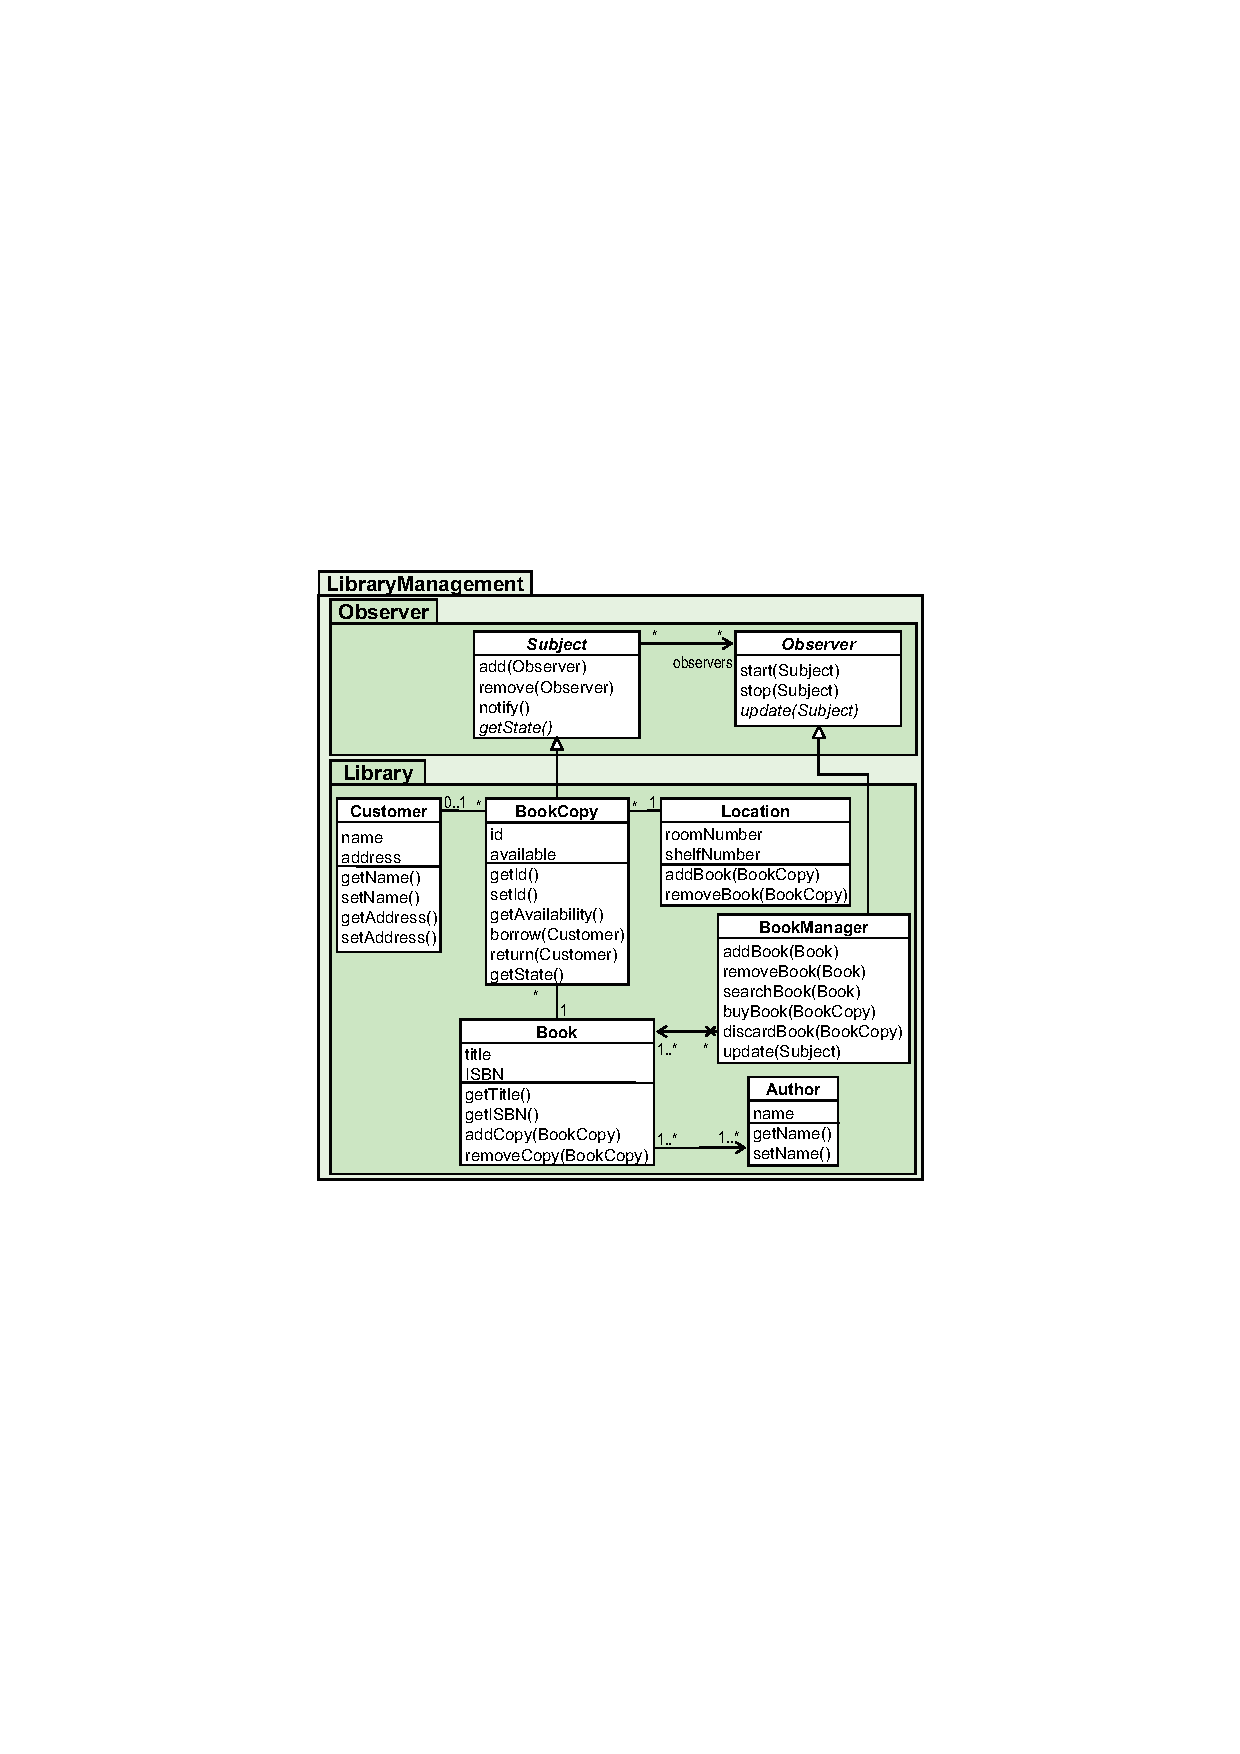
\includegraphics[width=0.7\textwidth]{figures/figure1}
	\caption{Sample figure}
	\label{fig:samplefigure_pdf}
\end{figure}


\section{Fonts}

When introducing important terms for the first time use \emph{emphasize}. For a consistent look and feel of proper names like {\cd} and {\uml{Observer}} pattern you may define macros in the main document \texttt{thesis.tex}.

\section{Code}

For short code fragments use the \textit{verbatim} environment.

\begin{verbatim}
//Start Program
System.out.println("Hello World!");
//End Program
\end{verbatim}

A much better alternative is the \textit{algorithm} environment (cf. Algorithm~\ref{alg:samplealgorithm}). This environment offers special formatting features for loops, operations and comments.

\begin{algorithm}[t]
\SetKwData{Left}{left}
\SetKwData{This}{this}
\SetKwData{Up}{up}
\SetKwFunction{Union}{Union}
\SetKwFunction{FindCompress}{FindCompress}
\SetKwInOut{Input}{input}
\SetKwInOut{Output}{output}

\Input{A bitmap $Im$ of size $w\times l$}
\Output{A partition of the bitmap}

\BlankLine

\emph{special treatment of the first line}\;
\For{$i\leftarrow 2$ \KwTo $l$}{
\emph{special treatment of the first element of line $i$}\;
\For{$j\leftarrow 2$ \KwTo $w$}{\label{forins}
\Left$\leftarrow$ \FindCompress{$Im[i,j-1]$}\;
\Up$\leftarrow$ \FindCompress{$Im[i-1,]$}\;
\This$\leftarrow$ \FindCompress{$Im[i,j]$}\;
\If(\tcp*[r]{O(\Left,\This)==1}){\Left compatible with \This}{\label{lt}
\lIf{\Left $<$ \This}{\Union{\Left,\This}}\;
\lElse{\Union{\This,\Left}\;}
}
\If(\tcp*[r]{O(\Up,\This)==1}){\Up compatible with \This}{\label{ut}
\lIf{\Up $<$ \This}{\Union{\Up,\This}}\;
\tcp{\This is put under \Up to keep tree as flat as possible}\label{cmt}
\lElse{\Union{\This,\Up}}\tcp*[r]{\This linked to \Up}\label{lelse}
}
}
\lForEach{element $e$ of the line $i$}{\FindCompress{p}}
}
\caption{Sample algorithm}\label{alg:samplealgorithm}
\end{algorithm}



%%%%%%%%%%%%%%%%%%%%%%%%%%%%%%%%%%%%%%%%%
%\chapter{Bibliographic Issues}
%\label{ch:bibliographic}
%%%%%%%%%%%%%%%%%%%%%%%%%%%%%%%%%%%%%%%%%
%\section{Literature Search}


\section{BibTeX}

BibTeX should be used for referencing. JabRef (an open source tool for Windows) is recommended for the management of references. 

The LaTeX source document of this pdf document provides you with different samples for references to journals~\cite{jour:B2BServices}, conference papers~\cite{proc:TheWebMLApproach}, books~\cite{book:umlatwork}, book chapters~\cite{incoll:ErhardKonrad1992}, electronic standards~\cite{man:BPEL}, dissertations~\cite{phdthesis:manuelWimmer}, masters' theses~\cite{mast:AUMLProfile}, and web sites~\cite{misc:BIGWebsite}. The respective BibTeX entries may be found in the file \texttt{references.bib}. For administration of the BibTeX references we recommend \url{http://www.citeulike.org} or JabRef for offline administration, respectively.


%%%%%%%%%%%%%%%%%%%%%%%%%%%%%%%%%%%%%%%%%
%%% BACKMATTER %%%%%%%%%%%%%%%%%%%%%%%%%%
%%%%%%%%%%%%%%%%%%%%%%%%%%%%%%%%%%%%%%%%%

\appendix

\bibliographystyle{plain}
\bibliography{references}

\end{document}
